\documentclass[11pt,a4paper,onecolumn,final]{article}

%Prevent text from hyphenation.
\usepackage[none]{hyphenat}
\usepackage{algpseudocode}

%Use this to import the generated modulation constellations
\usepackage{pdfpages}

%OT1 is the default font encoding of memoir class
%It is generally advised to put it before inputenc
\usepackage{kerkis}
\usepackage[T1]{fontenc}

%Input encoding for typing directly Greek characters
%Other values for the option: latin1, ascii, ansinew
%It is generally advised to put it before babel
\usepackage[utf8]{inputenc}

%MAIN Language the LAST one
\usepackage[english]{babel}

%\usepackage{kerkis}

%Package for displaying math
\usepackage{amsmath}

%Loading a superset of amsfonts
\usepackage{amssymb}

%Provides an enhanced version of \newtheorem
%1.Defines * for unnumbered environments
%2.Defines a proof environment
%3.Defines plain, definition, and remark theorem styles
\usepackage{amsthm}

%Allows text in eps files to be replaced with LATEX symbols
\usepackage{psfrag}

%An extension of the cite package, compatible with the IEEEtranN bibliography style
\usepackage[numbers,sort&compress]{natbib}

\makeatletter\let\c@lofdepth\relax\let\c@lotdepth\relax\makeatother
% \usepackage[small,bf,tight]{subfigure}
\usepackage{subcaption}

%Math symbols of the dsfont style. Enables the use of \mathds{}
\usepackage{dsfont}

%Defines several symbols in text mode (e.g. the \textreferencemark for use in the itemize environment)
\usepackage{textcomp}

%Enables the Ralph Smith's Formal Script font in math mode via the \mathscr{} command
\usepackage{mathrsfs}

\usepackage{geometry}
%PDF VIEW
\geometry{total={210mm,297mm},left=25mm,right=25mm,bindingoffset=0mm, top=25mm,bottom=25mm}
%PRINT
%\geometry{total={210mm,297mm},left=20mm,right=20mm,bindingoffset=10mm, top=25mm,bottom=25mm}

\usepackage[breaklinks=true,colorlinks=true,
linkcolor=blue,urlcolor=blue,citecolor=blue,% PDF VIEW
%linkcolor=black,urlcolor=black,citecolor=black,% PRINT
bookmarks=false,bookmarksopenlevel=2]{hyperref}

%Convenient language switch
\newcommand{\en}[1]{\foreignlanguage{english}{#1}}

%\newtheorem{definition}{Ορισμός}
\newtheorem{definition}{Definition}
\newtheorem{example}{Example}
\newtheorem{exercise}{Exercise}
%\newtheorem{lemma}{Λήμμα}
\newtheorem{lemma}{Lemma}
%\newtheorem{proof}{Proof}
\newtheorem{notation}{Notation}
\newtheorem{problem}{Problem}
%\newtheorem{proposition}{Πρόταση}
\newtheorem{proposition}{Proposition}
\newtheorem{remark}{Remark}
\newtheorem{solution}{Solution}
\newtheorem{summary}{Summary}
\newcommand{\argmax}{\arg\!\max}
%\addto\captionsgreek{\renewcommand{\chaptername}{Κεφάλαιο}}
%\addto\captionsgreek{\renewcommand{\tablename}{Πίνακας }}
%\addto\captionsgreek{\renewcommand{\proofname}{Απόδειξη }}

\makeatletter
%\renewcommand{\fnum@figure}{Σχήμα \thefigure}
%\renewcommand{\fnum@table}{Πίνακας \thetable}
\makeatother
\begin{document}

%COVER PAGE%%%%%%%%%%%%%%%%%%%%%%%%%%%%%%%%%%%%%%%%%%%%%%%%%%%%%%%%%%%%%%%%%%%%%

\thispagestyle{empty}
{\sffamily\centering\Large

\vspace{\fill}

{\Large Aristotle University of Thessaloniki\\
Department of Electrical and Computer Engineering}\\[0.5cm]


\vspace{2.0cm}

{\LARGE Antoniou, Antonios - 9482\\
Kaimakamidis, Anestis - 9627}

\vspace{3.5cm}

	
{\LARGE Parallel and Distributed Systems}\\[1em]

{\Large Comparing pthreads, openCilk and Multicilk}

\vspace{3.5cm}

%\vspace{\fill}

}

%%COVER PAGE%%%%%%%%%%%%%%%%%%%%%%%%%%%%%%%%%%%%%%%%%%%%%%%%%%%%%%%%%%%%%%%%%%%%%

\newpage

\section{Abstract}
\subsection{Symmetric Multiprocessing (SMP)}
Symmetric Multiprocessing, or SMP, is a programming paradigm meant for distributing a program’s workload across a machine’s threads, instead of the sequential execution of instructions, in the expense of added source code complexity. The concurrent processing is realized by the use of both shared and private entities in the context of each thread. In this paper, we will be taking a closer look at three ways of setting up a piece of SMP software: pthreads, openCilk and Multicilk.\\
\\
However, before getting into detail, it’s crucial that we clear up some terminology and basics of SMP. Since some of the variables -or more generally memory regions- are shared between threads (can be interchangeably called “processes” as well), there is need for a consistent methodology utilized to make sure that both access to and processing of them without being led to race conditions.
\subsection{Important terminology}
• \textbf{Race conditions}: A program is susceptible to race conditions, or race hazards, when the order in which threads execute the given instructions can have inconsistent influence on the outcome of the program.
There are two main ways of maintaining consistency:\\
• \textbf{Mutexes}: When a thread is about to update a variable -or entity- it obtains a lock designated for access to a certain memory space. When updating is over, the lock is released -or unlocked- again. While a mutex is locked, no other thread is allowed to update, or read a variable. In order to gain access to the mutex-ed variable, a thread must ask for it again, until it finds it an unlocked state.\\
• \textbf{Condition variables}: They work much like mutexes with a significant change in granting access to all threads. When a lock is unlocked after the successful update of a value, a signal is put out to all threads so that they can access it immediately. This means that no thread needs to persistently ask for permission to a variable until it is finally given to it.\\
• We wrap regions of the code that process an entity that’s shared among processes around some mutex logic. This region is oftentimes referred to as a \textbf{critical section}.
\section{Different multithreading schemes}
Pthreads makes use of condition variables for managing critical sections, while openCilk is limited to mutexes. However, one important advantage of the latter is work stealing. More specifically, when a pthread is created, it is very strictly assigned a certain piece of workload. Work stealing introduces flexibility and dynamic scheduling to the work assigned to all threads. This is more easily understood using a cilk\_for loop as an example.\\
\\
When a thread is done with the iteration of the loop assigned to it, it checks if any iteration is free. If so, it immediately starts executing it. So, thread with ID 0 could be executing the body of a loop for iteration $i=10$, while thread 1 could still be executing iteration $i=4$.\\
\\
On the other hand, Multicilk tries to take advantage of both software architectures. Cilk threads (often called cilks) are created, with each one of them having the permission to delegate some piece of their work to pthreads. This gives Multicilk the ability to use both work stealing and condition variables, depending on the region of the code the programmer needs to optimize. For that reason, we have constructed, roughly, the same algorithm for all three of the parallelization methods in order to compare their performances. Below are the specifics of each procedure.
\section{Brief description of the problem}
We will construct a problem that utilizes instructions for which both condition variables and work stealing makes sense, so that we can quantify their influence on the execution times. More specifically, our algorithm is a classic \textbf{producer-consumer} problem. We use a cyclical array that produces random seeds (we will call this number alpha). This seed is multiplied by random numbers to form an array of a constant user-given size. At this point, the producer has completed their work. Now it’s up to the consumers to take that array and perform a basic linear algebra operation on it. The operations we have programmed for the purposes of this project are axpy and a general sum of the elements of the array, sequentially, via pthreads and via openCilk. 
\subsection{Axpy}
Having two arrays, $x$ and $y$, axpy performs the operation:
\begin{equation}
y=\alpha\cdot x+y,
\end{equation}
where $\alpha$ is a constant value given to the operation by the program.
\subsection{Sum}
Sum takes an array $x$ and a similar $\alpha$ parameter and performs:
\begin{algorithmic}
\For{\texttt{i in size(x)}}
	\State $sum=sum+\alpha\cdot x[i]$
\EndFor
\end{algorithmic}
\section{Algorithm implementation}
\subsection{Pthreads and openCilk}
The program is written to work using a number of threads -we will call it $n$-. Let’s suppose $n=4$. For the first two implementations, this means $n^{2}=16$ threads will be utilized. All of them will be both producers and consumers. They will enter a for loop and produce-consume until a counter is reached. Every array that is produced and then consumed, increments that counter by one, obviously using condition variables or mutexes to maintain consistency and overall deterministic behavior. When the counter reaches a user-given constant, all threads are joined and the program returns.
\subsection{Multicilk}
For Multicilk, we took advantage of the ability for more detailed work assignment, while still maintaining some of the much-helpful concept of work stealing. So, $n$ cilks are invoked, and start producing arrays. Each one of them can use $n$ pthreads to consume their produced arrays. Again, on the completion of an arithmetic operation on an array, a counter is incremented, until a certain value is reached. Using the design above, we call the same number of threads as the simpler implementations, with a difference in the roles they take up.
\section{Testing}
\subsection{Test parameters}
The parameters given to the various resulting executables are:\\
• \textbf{n}: Essentially the root of the number of threads to be invoked, in the fashion that has been mentioned above\\
• \textbf{Size}: The size of each individual array, in elements.\\
• \textbf{Cases}: Number of arrays that must be produced and consumed.\\
• \textbf{Alpha}: The constant float value, used to perform both axpy and sum.\\
\subsection{Conducted tests}
For the purposes of our research, we conduct tests for various sizes, number of threads, and number of arrays to be produced and consumed.
\subsubsection{Pthreads vs openCilk}
Our main test consists of of \textbf{10 arrays} of \textbf{sizes 1000000, 2000000, and 5000000}. The \textbf{thread numbers} (n) are \textbf{2, 4, 6, 8, 12, and 16}. 

\begin{figure}
    \begin{subfigure}{.5\textwidth}
        \centering
        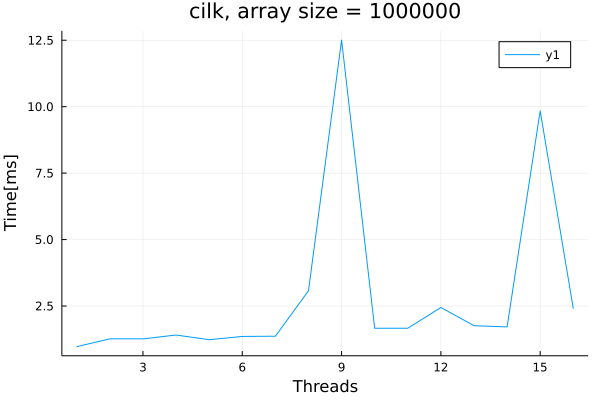
\includegraphics[width=.9\linewidth]{../data/image/method/cilk_1000000.png}
        \caption{openCilk - 1000000 elements}
    \end{subfigure}%
    \begin{subfigure}{.5\textwidth}
        \centering
        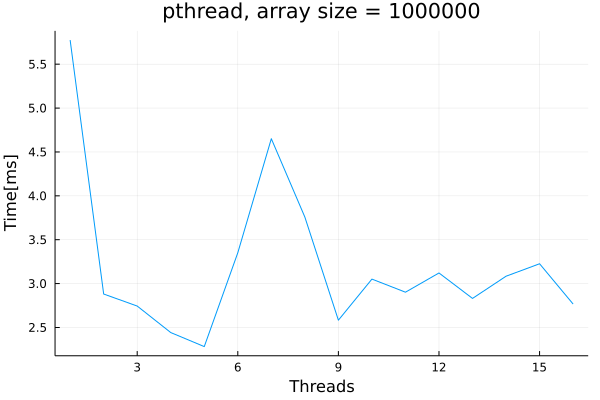
\includegraphics[width=.9\linewidth]{../data/image/method/pthread_1000000.png}
        \caption{pthread - 1000000 elements}
    \end{subfigure}
\end{figure}

\begin{figure}
    \begin{subfigure}{.5\textwidth}
        \centering
        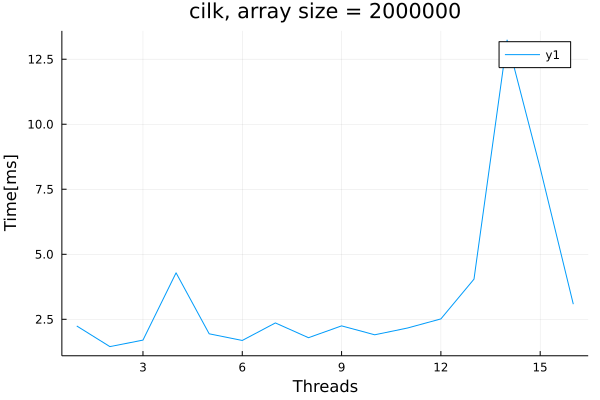
\includegraphics[width=.9\linewidth]{../data/image/method/cilk_2000000.png}
        \caption{openCilk - 2000000 elements}
    \end{subfigure}%
    \begin{subfigure}{.5\textwidth}
        \centering
        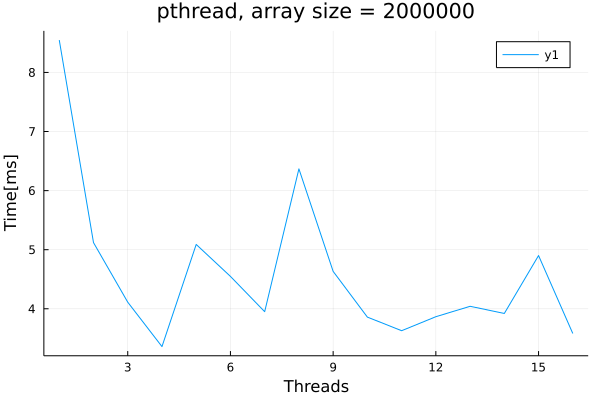
\includegraphics[width=.9\linewidth]{../data/image/method/pthread_2000000.png}
        \caption{pthread - 2000000 elements}
    \end{subfigure}
\end{figure}

\begin{figure}
    \begin{subfigure}{.5\textwidth}
        \centering
        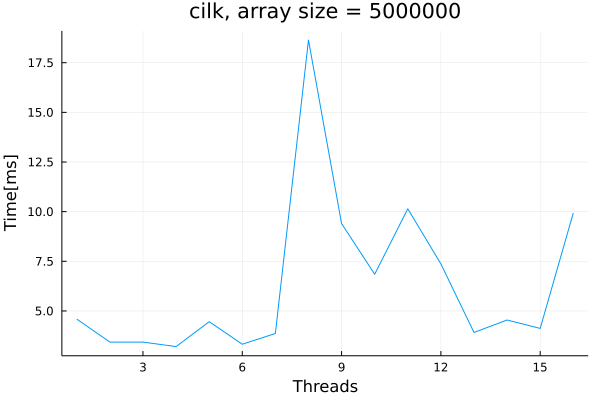
\includegraphics[width=.9\linewidth]{../data/image/method/cilk_5000000.png}
        \caption{openCilk - 5000000 elements}
    \end{subfigure}%
    \begin{subfigure}{.5\textwidth}
        \centering
        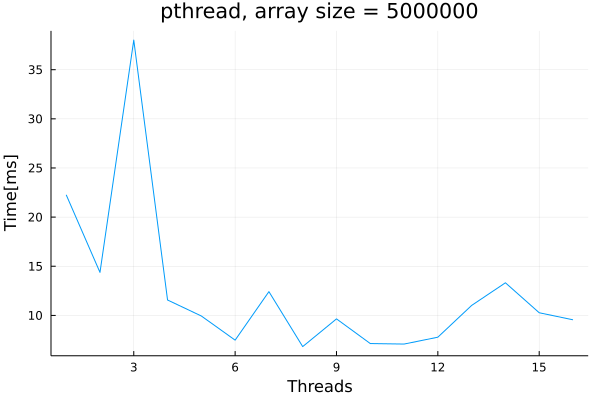
\includegraphics[width=.9\linewidth]{../data/image/method/pthread_5000000.png}
        \caption{pthread - 5000000 elements}
    \end{subfigure}
\end{figure}

We will observe the differences between the two schemes a little closer, for a \textbf{selected number of threads: 2, 4, 8, and 16.} 

\begin{figure}
    \begin{subfigure}{.5\textwidth}
        \centering
        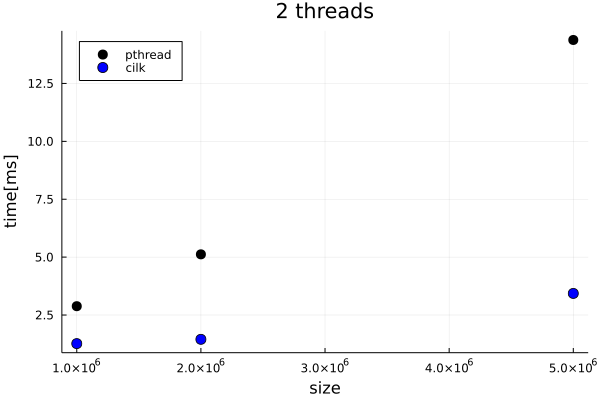
\includegraphics[width=.9\linewidth]{../data/image/thread/2-threads.png}
        \caption{Comparison for 2 threads}
    \end{subfigure}%
    \begin{subfigure}{.5\textwidth}
        \centering
        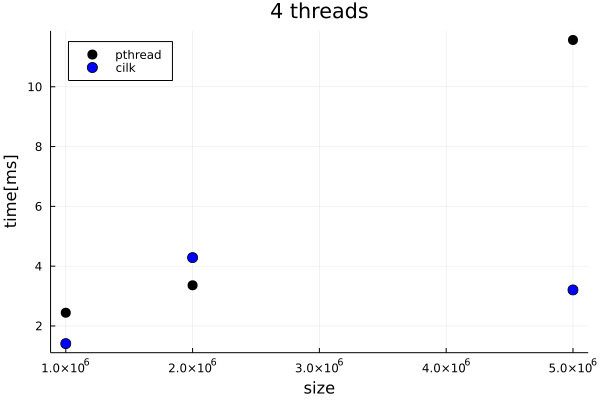
\includegraphics[width=.9\linewidth]{../data/image/thread/4-threads.png}
        \caption{Comparison for 4 threads}
    \end{subfigure}
\end{figure}

\begin{figure}
    \begin{subfigure}{.5\textwidth}
        \centering
        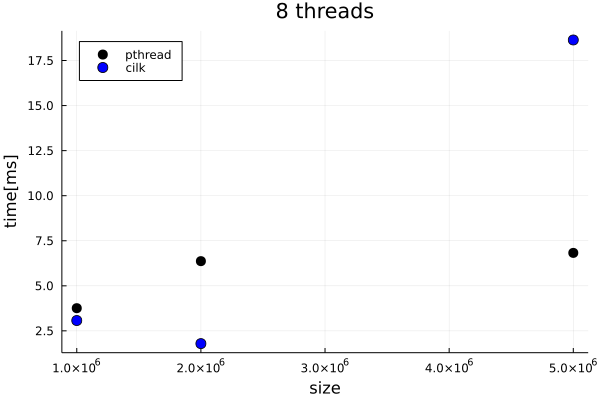
\includegraphics[width=.9\linewidth]{../data/image/thread/8-threads.png}
        \caption{Comparison for 8 threads}
    \end{subfigure}%
    \begin{subfigure}{.5\textwidth}
        \centering
        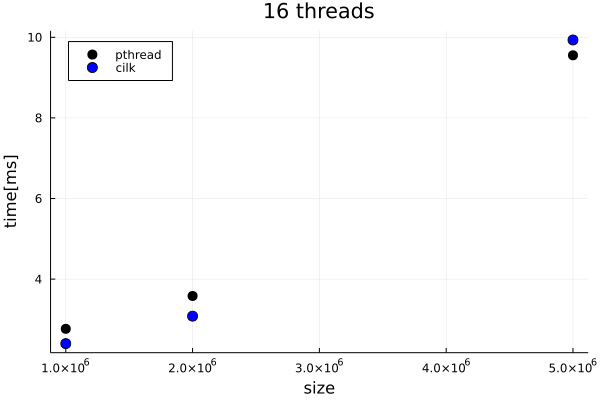
\includegraphics[width=.9\linewidth]{../data/image/thread/16-threads.png}
        \caption{Comparison for 16 threads}
    \end{subfigure}
\end{figure}

\subsubsection{Benchmarks between the three schemes}
The programs construct \textbf{10 arrays} of varying sizes, using $n=4$, which was shown to be the best performing parameter in the analysis above. For that parameter, we use arrays of \textbf{size 500000, 600000, 700000, 800000, 900000, 1000000, 2000000, 3000000, 4000000, and 5000000}.

\begin{figure}[p]
    \centering
    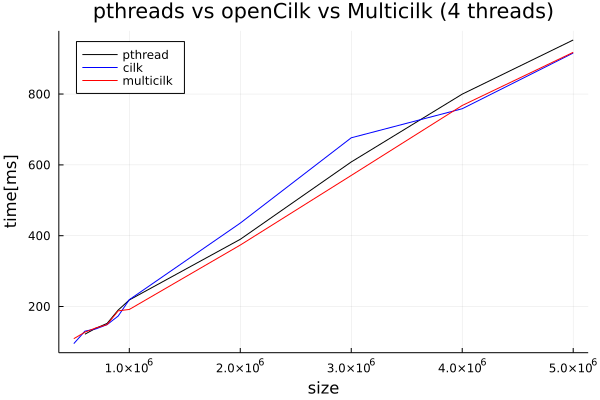
\includegraphics[scale=.5]{../data/image/benchmark/4-threads.png}
    \caption{Final comparison}
\end{figure}

\section{Conclusion}
The tests above show that openCilk's work stealing feature can offer more room for optimization, but less potential for deterministic behavior and predictability. All pthreads implementations seem to be scaling in a more predictable and linear manner, at least up until a number of threads that is in par with the specifications of the machine on which the tests were conducted.\\
\\
However, on the first batch of tests, for a large enough size, when work stealing actually makes sense, it is easy to see that openCilk is able to outperform pthreads, where the workload is statically assigned and prone to imbalance.\\
\\
Regarding the second batch, larger sizes and more threads than the ones natively built into the hardware lead openCilk to larger execution times, while more ideal conditions render openCilk capable of outperforming pthreads once again.\\
\\
Last, but not least, the \textbf{Multicilk comparison} leaves much to be desired. Generally speaking, the conducted tests are the perfect way for the average programmer to realize that no scheme, paradigm or design is a panacea. Each one of them needs to be carefully engineered and fit into a problem that is fit for its advantages and hides its disadvantages. Multicilk needs a large number of threads, a large enough problem, and most importantly a vast amount of data communication between underlying threads. Even so, one could be a little skeptical about its ease and merits of use. This would be the reason why there is little to no bibliography found on the matter \cite{pusapaty2022combining}.


% \renewcommand\bibname{\gr{Βιβλιογραφία}}
\bibliographystyle{IEEEtranN}
\en{\bibliography{citations}}

\end{document}
